% ----------------------------------------------------------------------------
% B.9 --- Spectral Scaling and the Projection Ontology
% From former B09, condensed
% ----------------------------------------------------------------------------
\subsection{Spectral Scaling and the Projection Ontology}
\label{subsec:spectral-scaling-projection-ontology}

Inertial mass is a spectral signature of projection visibility.
The non-injective projection $\Pi$ implies that each effective particle
corresponds to a large equivalence class of micro-configurations whose
stability eigenvalues measure the fiber weight.
The ratio
$m_p/m_e \approx \sqrt{\lambda_p/\lambda_e}$
is independent of the absolute action scale $\hbar_\chi$ and is
therefore a structurally protected invariant.

\begin{figure}[htbp]
  \centering
  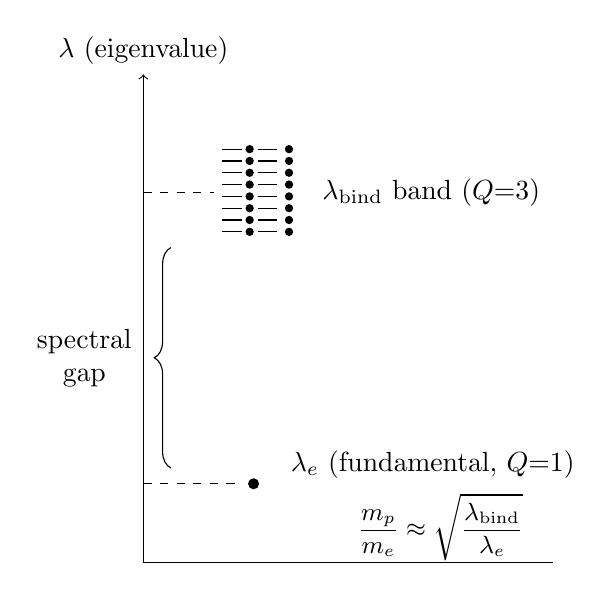
\begin{tikzpicture}[x=1cm,y=1cm]
    \draw[->] (0,0) -- (0,6.2)
      node[above] {$\lambda$ (eigenvalue)};
    \draw (0,0) -- (5.2,0);
    \fill (1.4,1.0) circle (2pt);
    \node[anchor=west] at (1.75,1.25)
      {$\lambda_e$ (fundamental, $Q{=}1$)};
    \foreach \y in
      {4.2,4.35,4.5,4.65,4.8,4.95,5.1,5.25} {
      \draw (1.0,\y) -- (1.25,\y);
      \fill (1.35,\y) circle (1.5pt);
      \draw (1.45,\y) -- (1.70,\y);
      \fill (1.85,\y) circle (1.5pt);
    }
    \node[anchor=west] at (2.15,4.7)
      {$\lambda_{\mathrm{bind}}$ band ($Q{=}3$)};
    \draw[decorate,
      decoration={brace,amplitude=6pt}]
      (0.35,1.2) -- (0.35,4.0)
      node[midway,xshift=-1.1cm,align=center]
        {spectral\\gap};
    \draw[dashed] (0,1.0) -- (1.2,1.0);
    \draw[dashed] (0,4.7) -- (0.9,4.7);
    \node[anchor=west,align=left] at (2.6,0.45)
      {\small $\displaystyle
        \frac{m_p}{m_e}
        \approx
        \sqrt{\frac{\lambda_{\mathrm{bind}}}
                   {\lambda_e}}$};
  \end{tikzpicture}
  \caption{Spectral gap in the stability spectrum of
    $\mathcal{L}_{\mathrm{sol}}$: elementary mode
    $\lambda_e$ separated from binding-mode band
    $\lambda_{\mathrm{bind}}$.}
  \label{fig:spectral-gap}
\end{figure}
